%-------------------------
% Rodrigo Arsenio - CV
% Based on: https://github.com/jakegut/resume (MIT)
% Build: tools/tectonic.exe CV_RodrigoArsenio.tex
%------------------------

\documentclass[a4paper,11pt]{article}

\usepackage{latexsym}
\usepackage[empty]{fullpage}
\usepackage{titlesec}
\usepackage{marvosym}
\usepackage[usenames,dvipsnames]{color}
\usepackage{verbatim}
\usepackage{enumitem}
\usepackage[hidelinks]{hyperref}
\usepackage{fancyhdr}
\usepackage[english]{babel}
\usepackage{tabularx}
\usepackage{graphicx}

\pagestyle{fancy}
\fancyhf{}
\fancyfoot{}
\renewcommand{\headrulewidth}{0pt}
\renewcommand{\footrulewidth}{0pt}

% Adjust margins
\addtolength{\oddsidemargin}{-0.5in}
\addtolength{\evensidemargin}{-0.5in}
\addtolength{\textwidth}{1in}
\addtolength{\topmargin}{-.5in}
\addtolength{\textheight}{1.0in}

\urlstyle{same}

\raggedbottom
\raggedright
\setlength{\tabcolsep}{0in}

% Sections formatting
\titleformat{\section}{
  \vspace{-4pt}\scshape\raggedright\large
}{}{0em}{}[\color{black}\titlerule \vspace{-5pt}]

%-------------------------
% Custom commands
\newcommand{\resumeItem}[1]{
  \item\small{
    {#1 \vspace{-2pt}}
  }
}

\newcommand{\resumeSubheading}[4]{
  \vspace{-2pt}\item
    \begin{tabular*}{0.97\textwidth}[t]{l@{\extracolsep{\fill}}r}
      \textbf{#1} & #2 \\
      \textit{\small#3} & \textit{\small #4} \\
    \end{tabular*}\vspace{-7pt}
}

\newcommand{\resumeProjectHeading}[2]{
    \item
    \begin{tabular*}{0.97\textwidth}{l@{\extracolsep{\fill}}r}
      \small#1 & #2 \\
    \end{tabular*}\vspace{-7pt}
}

\renewcommand\labelitemii{$\vcenter{\hbox{\tiny$\bullet$}}$}

\newcommand{\resumeSubHeadingListStart}{\begin{itemize}[leftmargin=0.15in, label={}]}
\newcommand{\resumeSubHeadingListEnd}{\end{itemize}}
\newcommand{\resumeItemListStart}{\begin{itemize}}
\newcommand{\resumeItemListEnd}{\end{itemize}\vspace{-5pt}}

%-------------------------------------------
\begin{document}

%----------HEADING----------
\begin{minipage}[c]{0.20\textwidth}
    \flushleft
    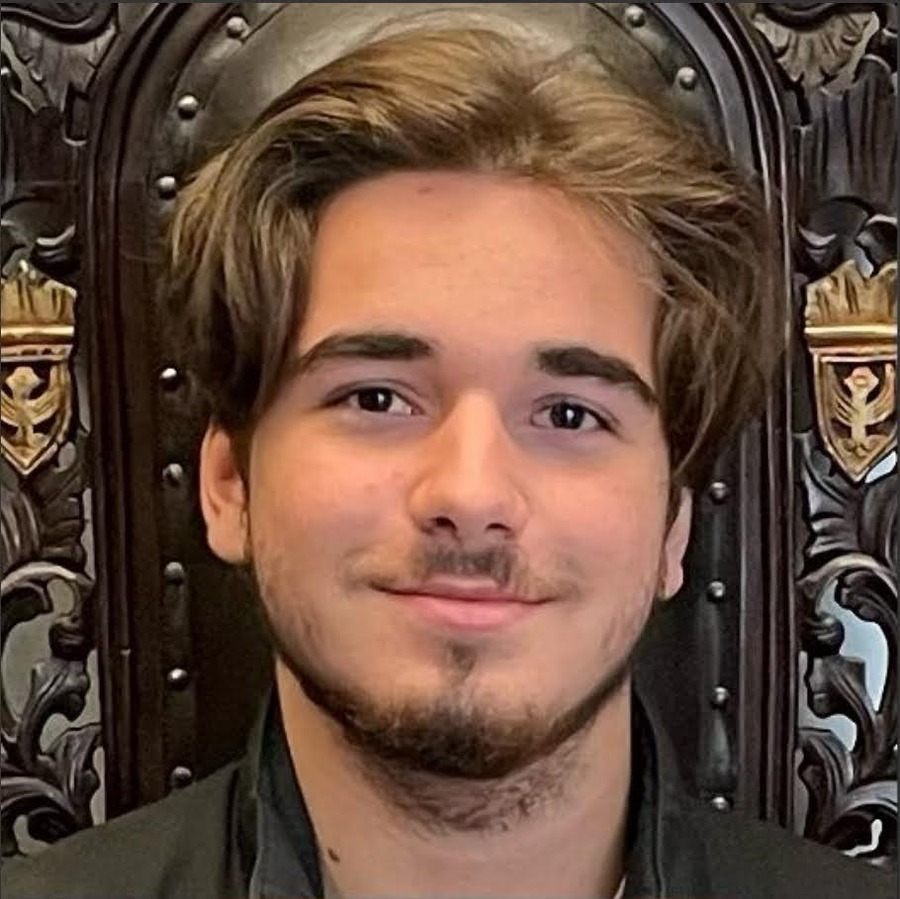
\includegraphics[width=3.5cm,height=3.5cm,keepaspectratio]{photo.jpg}
\end{minipage}%
\hfill
\begin{minipage}[c]{0.76\textwidth}
    \begin{center}
    {\Huge \scshape Rodrigo Ars\'enio} \\ \vspace{4pt}
    \small Charneca da Caparica, Portugal \\ \vspace{2pt}
    \small +351 961 935 508 $|$
    \href{mailto:rodrigo.m.arsenio@gmail.com}{\underline{rodrigo.m.arsenio@gmail.com}} \\ \vspace{2pt}
    \small \href{https://linkedin.com/in/rodrigo-arsenioo}{\underline{linkedin.com/in/rodrigo-arsenioo}} $|$
    \href{https://github.com/RodrigoArsenioo}{\underline{github.com/RodrigoArsenioo}}
    \end{center}
\end{minipage}

%-----------PROFILE-----------
\section{Profile}
 \begin{itemize}[leftmargin=0.15in, label={}]
    \small{\item{
Master's student in Computer Science and Engineering (Security and Privacy) at NOVA
FCT with professional experience shipping a production HTML5 game as part of a small
remote team.
Comfortable across the stack, from Svelte/WebGL frontends to Node.js tooling and
Java/Spring backends, with current research work on LLM-based text anonymization.
    }}
 \end{itemize}

%-----------EDUCATION-----------
\section{Education}
  \resumeSubHeadingListStart
    \resumeSubheading
      {Master's in Computer Science and Engineering}{Sep. 2025 -- July 2027 (expected)}
      {NOVA School of Science and Technology (FCT NOVA)}{Caparica, Portugal}
      \resumeItemListStart
        \resumeItem{Specialization in Security and Privacy, secondary concentration in Trustworthy Software Development}
        \resumeItem{Current average: 15.39/20 (first year completed, 60 ECTS)}
        \resumeItem{Selected coursework: Systems Privacy (19), Advanced Applied Cryptography (17), Software Security (16), Software Verification (16), Distributed Algorithms (16)}
        \resumeItem{MSc thesis (ongoing): \emph{Creating a risk-based unstructured data anonymization method using LLMs}, supervised by Prof.\ Kevin Gallagher. Developing LLM-powered anonymization of unstructured court documents, guided by risk-based anonymization metrics, so courts can publish decisions without exposing personal data}
      \resumeItemListEnd
    \resumeSubheading
      {Bachelor's in Computer Science and Engineering}{Sep. 2022 -- July 2025}
      {NOVA School of Science and Technology (FCT NOVA)}{Caparica, Portugal}
      \resumeItemListStart
        \resumeItem{Core foundations: data structures and algorithms, object-oriented programming, operating systems, databases, computer networks, distributed systems, software engineering, and artificial intelligence}
      \resumeItemListEnd
    \resumeSubheading
      {High School}{Sep. 2019 -- July 2022}
      {Col\'egio Guadalupe}{Verdizela, Portugal}
      \resumeItemListStart
        \resumeItem{Final average: 17.44/20}
      \resumeItemListEnd
  \resumeSubHeadingListEnd

%-----------EXPERIENCE-----------
\section{Experience}
  \resumeSubHeadingListStart
    \resumeSubheading
      {Web Game Developer}{June 2026 -- Present}
      {Independent three-person studio}{Remote}
      \resumeItemListStart
        \resumeItem{Co-developed and shipped a production HTML5 game to a high-traffic online gaming platform}
        \resumeItem{Built the gameplay UI and animation flows in Svelte and TypeScript on a PixiJS (WebGL) rendering pipeline}
        \resumeItem{Led the platform certification process and the release tooling (reproducible builds, automated pre-release checks)}
      \resumeItemListEnd
    \resumeSubheading
      {Full-Stack Developer, EmberShields}{Jan. 2025 -- July 2025}
      {Land management platform, NOVA FCT and municipal partnership}{Caparica, Portugal}
      \resumeItemListStart
        \resumeItem{Built a web and mobile platform for sustainable land management in a 5-person team with local municipal authorities, graded 18/20 (12 ECTS)}
        \resumeItem{Worked on GeoJSON mapping, offline-capable field data collection, JWT authentication, and role-based access control. Stack: Flutter, Spring Boot, PostgreSQL, Docker}
      \resumeItemListEnd
  \resumeSubHeadingListEnd

%-----------TECHNICAL SKILLS-----------
\section{Technical Skills}
 \begin{itemize}[leftmargin=0.15in, label={}]
    \small{\item{
     \textbf{Programming Languages}{: Java (primary), Python, JavaScript/TypeScript, C, OCaml, SQL, HTML/CSS} \\
     \textbf{Frameworks and Libraries}{: Spring, Node.js, Svelte, PixiJS (WebGL), RESTful APIs} \\
     \textbf{Developer Tools}{: Git/GitHub, Docker, Bash, SSH, Google Cloud Platform, Maven, IntelliJ IDEA, VS Code, \LaTeX} \\
     \textbf{Languages}{: Portuguese (native), English (fluent), Spanish (intermediate)}
    }}
 \end{itemize}

%-----------INTERESTS-----------
\section{Interests}
 \begin{itemize}[leftmargin=0.15in, label={}]
    \small{\item{PC building and performance tuning, from component selection to overclocking, undervolting and cooling optimization. Modding and tweaking software to understand how it works and make it run better.}}
 \end{itemize}

%-------------------------------------------
\end{document}
